
%(BEGIN_QUESTION)
% Copyright 2010, Tony R. Kuphaldt, released under the Creative Commons Attribution License (v 1.0)
% This means you may do almost anything with this work of mine, so long as you give me proper credit

The so-called {\it Claus process} is widely used to convert hydrogen sulfide gas (H$_{2}$S) into elemental sulfur (S), turning a waste product of oil refining into a valuable feedstock for chemical processes.  The conversion takes place in two steps, shown by these (unbalanced) chemical reactions:

$$\hbox{H}_2\hbox{S} + \hbox{O}_2 \rightarrow \hbox{SO}_2 + \hbox{H}_2\hbox{O} \hskip 30pt \Delta H = -518.8 \hbox{ kJ mol}^{-1}$$

$$\hbox{H}_2\hbox{S} + \hbox{SO}_2 \rightarrow \hbox{S} + \hbox{H}_2\hbox{O} \hskip 35pt \Delta H = -142.8 \hbox{ kJ mol}^{-1}$$

\vskip 10pt

A simplified PFD of the Claus process appears here:

$$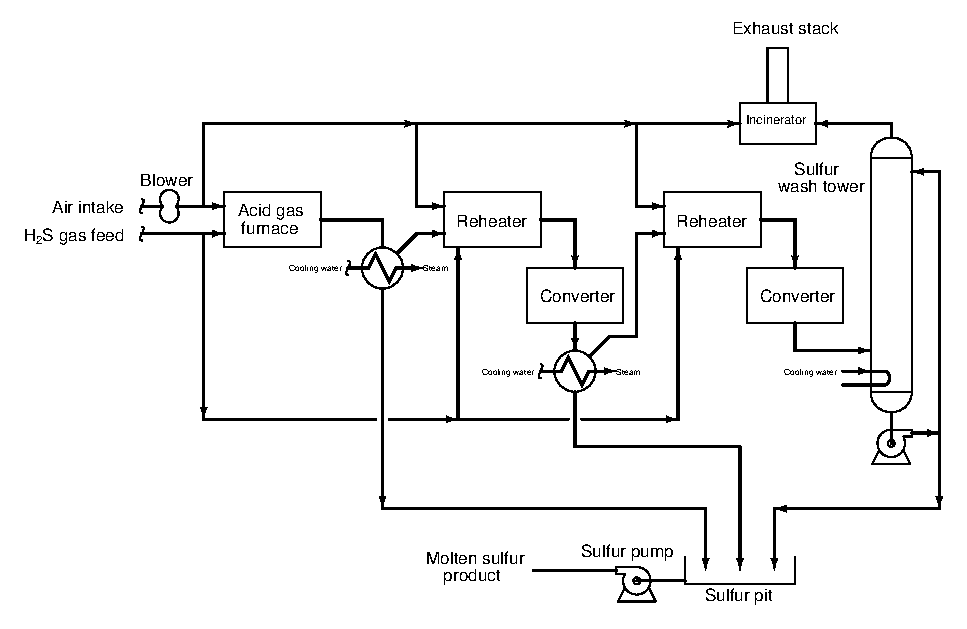
\includegraphics[width=15.5cm]{i03726x01.eps}$$

\noindent
Determine the following:

\begin{itemize}
\item{} Where each of the two chemical reactions occurs in the PFD.
\item{} The meaning of the $\Delta H$ values stated next to each equation.
\item{} Which of the two heat exchangers transfers more heat energy than the other.
\item{} The principal danger of H$_{2}$S gas as it relates to human health.
\item{} The probable types and locations of analytical transmitters in this process, and how their measurements might be used for control.
\item{} Potential pollutants emitted by this process into the atmosphere.
\end{itemize}

\vskip 20pt \vbox{\hrule \hbox{\strut \vrule{} {\bf Suggestions for Socratic discussion} \vrule} \hrule}

\begin{itemize}
\item{} Identify suitable flowmeter technologies for each of the process flows shown in this PFD.  Note that molten sulfur is hot (about 240 $^{o}$F), viscous, and solidifies quickly when cooled to ambient temperature.
\item{} Identify pipes carrying fluids into and out of various vessels in this process, and identify whether the temperature of the incoming or outgoing flow will be greater.  Explain why, in each case.
\end{itemize}

\underbar{file i03726}
%(END_QUESTION)





%(BEGIN_ANSWER)


%(END_ANSWER)





%(BEGIN_NOTES)

\begin{itemize}
\item{} Where each of the two chemical reactions occurs in the PFD.  {\it Both reactions take place in the acid gas furnace, and in the reheaters.  The second reaction mostly occurs in the two converter vessels.}
\vskip 10pt
\item{} The meaning of the $\Delta H$ values stated next to each equation. {\it The negative value means both reactions are exothermic, the first releasing much more heat than the second.  Another clue to the exothermic nature of these reactions is the presence of cooling water heat exchangers after every reactor.}
\vskip 10pt
\item{} Which of the two heat exchangers transfers more heat energy than the other.  {\it The first heat exchanger (after the acid gas furnace) because it handles most of the first reaction than the others, which is the most exothermic.}
\vskip 10pt
\item{} The principal danger of H$_{2}$S gas as it relates to human health.  {\it Hydrogen sulfide paralyzes the nervous system in low concentrations.}
\vskip 10pt
\item{} The probable types and locations of analytical transmitters in this process, and how their measurements might be used for control.  {\it Definitely SO$_{2}$ analyzers following the converters, to indicate how thorough the second reaction proceeded.  Possibly also H$_{2}$S analyzers as well to secondarily indicate reaction completeness.  Ambient air H$_{2}$S analyzers scattered throughout the unit for personnel safety.}
\vskip 10pt
\item{} Potential pollutants emitted by this process into the atmosphere.  {\it Unreacted H$_{2}$S and SO$_{2}$.}
\end{itemize}

\vskip 10pt

Details on process chemistry taken from pages 323-324 of {\it Shreve's Chemical Process Industries}, fifth edition, by George T. Austin.

\vfil \eject

\noindent
{\bf Prep Quiz:}

The {\it Claus process} is used in industry to:

\begin{itemize}
\item{} Measure the concentration of NO$_{x}$ in furnace stack gases
\vskip 5pt 
\item{} Condense liquid impurities from gas samples going into analyzers
\vskip 5pt 
\item{} Extract elemental sulfur from hydrogen sulfide gas in oil refining
\vskip 5pt 
\item{} Produce water vapor and carbon dioxide from benezene liquid
\vskip 5pt 
\item{} Neutralize the pH of wastewater in municipal treatment facilities
\vskip 5pt 
\item{} Split water molecules into hydrogen and oxygen gas streams
\vskip 5pt 
\item{} Deliver gifts to good little boys and girls via an obese elf
\end{itemize}



\vfil \eject

\noindent
{\bf Summary Quiz:}

The $\Delta H$ values appearing to the right of a chemical equation represent:

\begin{itemize}
\item{} The net energy released or absorbed by the reaction 
\vskip 5pt 
\item{} The (total) number of moles of reaction products
\vskip 5pt 
\item{} The financial cost of this reaction, in US dollars per mole
\vskip 5pt 
\item{} The (total) number of moles of reactants 
\vskip 5pt 
\item{} The pH value of the reaction products, assuming they are liquid
\vskip 5pt 
\item{} Whether or not the reaction is thermodynamically reversible
\end{itemize}


%INDEX% Process: sulfur recovery from H2S gas (Claus process)

%(END_NOTES)

